\documentclass[simplex.tex]{subfiles}
% NO NEED TO INPUT PREAMBLES HERE
% packages are inherited; you can compile this on its own

\onlyinsubfile{
\title{NeuroData SIMPLEX Report: Subfile}
}

\begin{document}
\onlyinsubfile{
\thispagestyle{empty}


%%%% Publications
\bibliographystyle{IEEEtran}
\begin{spacing}{0.5}
\nocite{*}
{\footnotesize	\bibliography{simplex}}
\end{spacing}
%%%% End Publications
}

\subsection{LOL}



As you may recall from last month, we successfully proved that LOL outperforms PCA essentially always when performing a linear dimensionality reduction prior to classification.  This month we generate simulation results supporting those theoretical claims (see Figure \ref{fig:LOL}).



\begin{figure}[h!]
\begin{cframed}
\centering
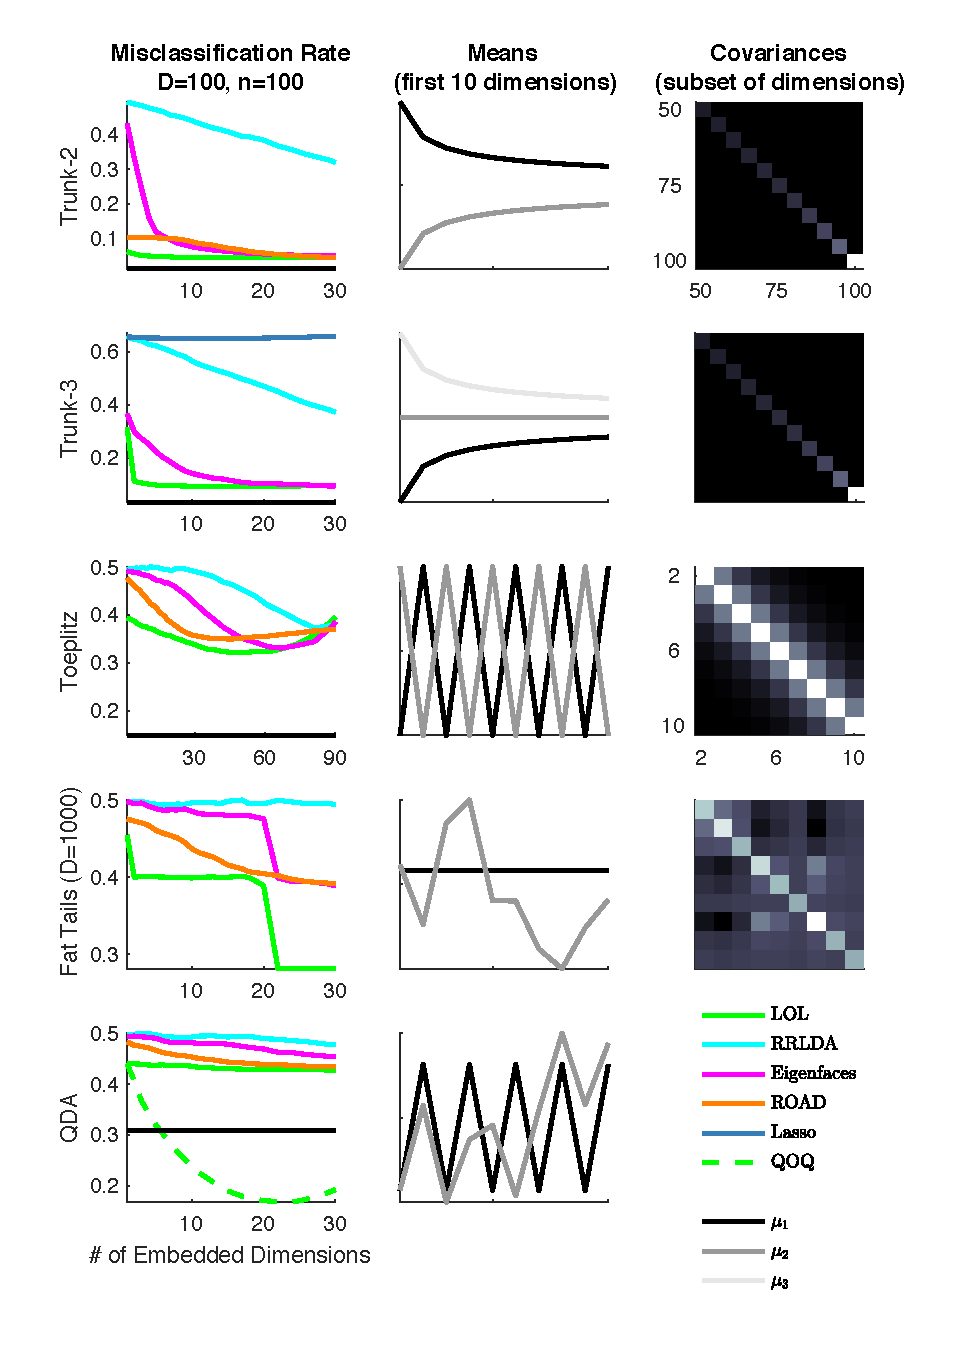
\includegraphics[width=0.7\textwidth]{../../figs/plot_all.pdf}
\caption{
LOL outperforms other linear classifiers in a wide variety of settings, including those for which we have proven LOL should (rows 1 and 3), and those beyond our current theoretical grasp (rows 2, 4, and 5). This is true regardless of the dimensionality into which we embed.
}
\label{fig:LOL}
\end{cframed}
\end{figure}

\end{document}
